\subsection{Experimental Setup}
\label{subsec:experimental-setup}

The experiments are designed as a controlled diagnostic study rather than an
exhaustive OOD benchmark. Section~\ref{sec:method} argues that optimizer choice
can change the ID geometry fingerprint \(G(h,W)\), and that downstream detector
families respond according to the geometry channels they read. We therefore
organize the experiments around three linked questions: whether weight-decay
coupling changes penultimate geometry, whether detector families inherit those
changes through different readout channels, and whether ID geometry can guide
detector diagnostics before OOD validation.

\textbf{Placeholder status.}
The numeric values in this section are synthetic placeholders used only to
stabilize the paper layout and figure/table pipeline. They are not experimental
evidence and must be replaced with measured values before submission.

We use CIFAR-10 as the primary ID dataset and evaluate near-OOD and far-OOD
settings separately. The main architecture families are non-residual VGG-style
CNNs, residual ResNet/WideResNet models, and modern ConvNeXt backbones.
Transformer-based architectures such as ViT and Swin are reserved for appendix
robustness experiments, where pretraining, normalization layers, and token-based
representations may change how optimizer effects appear. The optimizer set is
SGD, SGDW, Adam, and AdamW, with an AdamW-to-Adam interpolation used as an
optional mechanism sweep at fixed total weight decay.

Detector families include logit-based scores, raw and L2-normalized distance
scores, local-neighborhood scores, and DDU-style Gaussian feature-density / GMM
scores. Angular, prototype, and subspace diagnostics are included only when
their score conventions and implementations are fixed; otherwise, they are
treated as extended or appendix probes. All detector scores are oriented so that
larger values are more ID-like before AUROC, AUPR-IN, and FPR95 are computed.
Geometry is computed from ID training features unless otherwise stated.

\begin{table}[t]
\caption{SYNTHETIC PLACEHOLDER -- DO NOT REPORT as results. Experimental
protocol matrix specifying the planned prediction-driven evaluation structure.}
\label{tab:exp-protocol-matrix}
\begin{center}
\footnotesize
\setlength{\tabcolsep}{4pt}
\renewcommand{\arraystretch}{1.15}
\begin{tabular}{@{}p{0.18\textwidth}p{0.30\textwidth}p{0.42\textwidth}@{}}
\toprule
Component & Main setting & Purpose \\
\midrule
ID data & CIFAR-10; optional CIFAR-100 appendix & Controlled ID geometry measurement \\
OOD data & CIFAR-100, TinyImageNet, SVHN, MNIST & Near/far detector response \\
Architecture & VGG-style, ResNet/WideResNet, ConvNeXt & Inductive-bias robustness \\
Appendix architecture & ViT, Swin & Transformer/pretraining robustness \\
Optimizers & SGD, SGDW, Adam, AdamW & Adaptivity and weight-decay coupling \\
Mechanism sweep & AdamW\(\rightarrow\)Adam interpolation & Coupling-axis test \\
Logit scores & MSP, MaxLogit, Energy & Confidence/margin readouts \\
Feature scores & Mahalanobis, kNN, DDU-style Gaussian feature-density / GMM & Distance, neighborhood, density readouts \\
Diagnostics & L2, shrinkage, diagonal/tied covariance, PCA & Radial, covariance, and subspace channels \\
Metrics & Accuracy, NLL, ECE, AUROC, AUPR-IN, FPR95 & ID quality and OOD separation \\
Geometry & NC0--NC3, norm stats, eigenspectrum, effective rank & ID geometry fingerprint \\
\bottomrule
\end{tabular}
\end{center}
\end{table}


This setup is intended to separate two questions that are often conflated. First,
do optimizers with comparable ID performance induce different penultimate
geometry? Second, do detector families respond to those geometry differences in
a way that matches their readout channel? The following subsections answer these
questions without treating the result as a global optimizer ranking.

\subsection{Weight-Decay Coupling Changes Penultimate Geometry}
\label{subsec:wd-coupling-changes-geometry}

We first test whether weight-decay coupling acts as a geometry intervention. The
main mechanism sweep interpolates between AdamW and Adam while keeping the total
weight decay fixed. The interpolation parameter \(\gamma\) controls the fraction
of weight decay applied in the coupled gradient path: \(\gamma=0\) corresponds
to AdamW and \(\gamma=1\) corresponds to Adam. If coupling changes the update
geometry, then ID accuracy may remain comparable while NC metrics, feature-norm
statistics, covariance spectra, and detector behavior move along the coupling
axis.

Figure~\ref{fig:wd-coupling-interpolation} gives the planned visualization. The
left panel tracks ID accuracy, the middle panel tracks geometry summaries, and
the right panel tracks detector-family behavior. The intended evidence is not
that Adam or AdamW is universally better, but that the representation geometry
changes systematically as the optimizer moves from decoupled to coupled weight
decay.

\begin{figure}[t]
\centering
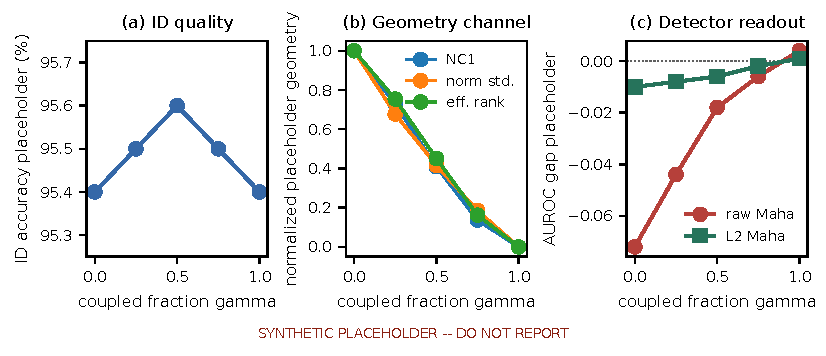
\includegraphics[width=\linewidth]{figures/fig2_wd_coupling_interpolation.pdf}
\caption{SYNTHETIC PLACEHOLDER -- DO NOT REPORT. Placeholder layout for the
AdamW-to-Adam interpolation experiment. The plotted values are synthetic and
must be replaced by measured results. The intended test is whether geometry and
detector behavior move along the weight-decay-coupling axis even when ID
accuracy remains comparable.}
\label{fig:wd-coupling-interpolation}
\end{figure}

\begin{table}[t]
\caption{SYNTHETIC PLACEHOLDER -- DO NOT REPORT. Summary for the
AdamW-to-Adam interpolation. These values are layout placeholders only and must
be replaced by measured results.}
\label{tab:dummy-interpolation-summary}
\begin{center}
\footnotesize
\setlength{\tabcolsep}{5pt}
\renewcommand{\arraystretch}{1.15}
\begin{tabular}{@{}cccccc@{}}
\toprule
\(\gamma\) & ID Acc. & NC1 & Norm std. & Eff. rank & Near AUROC gap \\
\midrule
0.00 & 95.4 & 0.081 & 1.42 & 38.0 & -0.072 \\
0.25 & 95.5 & 0.069 & 1.21 & 34.5 & -0.044 \\
0.50 & 95.6 & 0.055 & 1.04 & 30.2 & -0.018 \\
0.75 & 95.5 & 0.043 & 0.89 & 26.1 & -0.006 \\
1.00 & 95.4 & 0.037 & 0.77 & 23.8 &  0.004 \\
\bottomrule
\end{tabular}
\end{center}
\end{table}


We also compare the size of the coupled-versus-decoupled gap in adaptive and
non-adaptive optimizers. Let
\[
    \Delta_{\mathrm{nonadapt}}
    =
    d\bigl(G_{\mathrm{SGD}},G_{\mathrm{SGDW}}\bigr),
    \qquad
    \Delta_{\mathrm{adapt}}
    =
    d\bigl(G_{\mathrm{Adam}},G_{\mathrm{AdamW}}\bigr),
\]
where \(d(\cdot,\cdot)\) is a standardized distance over the ID geometry
fingerprint. The same comparison is computed for detector-family outputs. If
the adaptive preconditioner amplifies the effect of coupling, then the
Adam--AdamW gap should be larger than the SGD--SGDW gap under matched training
conditions.

\begin{figure}[t]
\centering
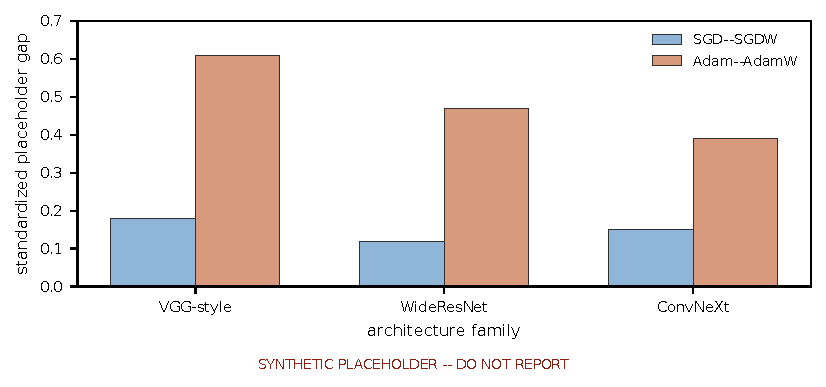
\includegraphics[width=\linewidth]{figures/fig3_adaptive_coupling_gap.pdf}
\caption{SYNTHETIC PLACEHOLDER -- DO NOT REPORT. Placeholder layout for comparing
the Adam--AdamW gap with the SGD--SGDW gap. Values are synthetic placeholders.
The intended figure compares standardized geometry distances and detector-family
distances across architecture families.}
\label{fig:adaptive-coupling-gap}
\end{figure}

If ID accuracy changes strongly along the interpolation, the sweep should be
interpreted as a hyperparameter sensitivity study rather than a clean mechanism
test. If ID accuracy is stable but geometry does not move, then weight-decay
coupling is not the dominant geometry intervention in that setting.

\subsection{Detector Families Respond Through Different Readout Channels}
\label{subsec:detector-readout-channel-response}

We next ask whether detector families inherit optimizer-induced geometry changes
uniformly. The compatibility view predicts that they should not. Logit-based
scores read output confidence and margins; raw Mahalanobis and raw kNN read
radial distance, class separation, and local feature-bank structure;
DDU-style Gaussian feature-density / GMM scores read covariance and density; and
angular or subspace diagnostics read prototype and residual structure.

Figure~\ref{fig:detector-family-delta-heatmap} reports the planned
optimizer-relative AUROC gap heatmap. The reference is the matched SGD anchor
within each architecture and dataset. Positive values indicate that the detector
family improves relative to the anchor, and negative values indicate
degradation. The purpose of this figure is not to declare a winning optimizer.
The purpose is to show whether the same representation remains compatible with
some readouts while becoming less compatible with others.

\begin{figure}[t]
\centering
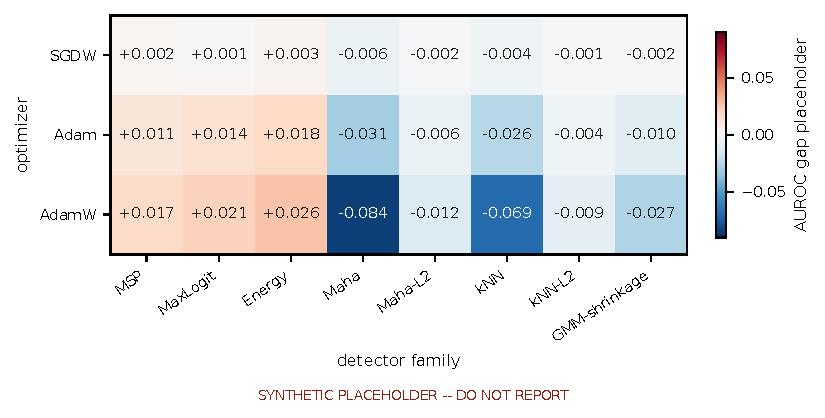
\includegraphics[width=\linewidth]{figures/fig4_detector_family_delta_heatmap.pdf}
\caption{SYNTHETIC PLACEHOLDER -- DO NOT REPORT. Placeholder detector-family
AUROC gap heatmap. Values are synthetic placeholders. The intended result format
compares logit, raw distance, L2 distance, Gaussian density, angular, and
subspace readouts relative to a matched SGD anchor.}
\label{fig:detector-family-delta-heatmap}
\end{figure}

A useful diagnostic pattern is a split between logit and feature readouts. If
logit scores remain stable while raw feature-distance scores degrade, the
optimizer has not produced a uniformly worse model. Instead, it has produced a
representation that is less compatible with the raw distance channel. If all
detectors degrade together, the result is more likely to reflect a broad model
quality issue rather than a geometry--detector compatibility effect.

\subsection{Diagnostic Controls Localize Geometry Channels}
\label{subsec:diagnostic-controls-localize-channels}

We then use detector-side controls to localize which geometry channel carries a
detector gap. These controls are diagnostic interventions, not proposed universal
fixes. L2 normalization removes the radial feature-norm channel; tied, diagonal,
and shrinkage covariance variants probe covariance estimation and conditioning;
and PCA or residual-subspace diagnostics separate principal ID directions from
residual directions.

The radial-channel diagnostic compares raw Mahalanobis and raw kNN against their
L2-normalized counterparts using the same checkpoints, ID feature bank, OOD
datasets, and score direction convention. Recovery after L2 normalization
indicates that the raw detector gap is carried by radial or norm-coupled
geometry.

\begin{figure}[t]
\centering
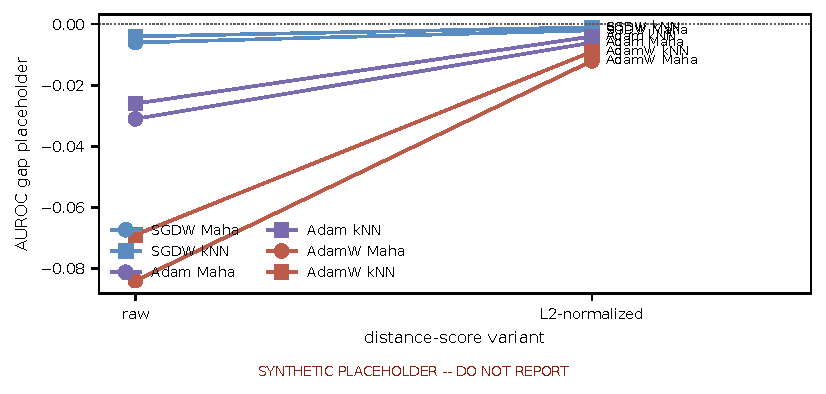
\includegraphics[width=\linewidth]{figures/fig5_l2_recovery_paths.pdf}
\caption{SYNTHETIC PLACEHOLDER -- DO NOT REPORT. Placeholder raw-to-L2 recovery
plot for Mahalanobis and kNN. Values are synthetic placeholders. Strong movement
toward zero after L2 normalization would implicate a radial or norm-coupled
failure channel.}
\label{fig:l2-recovery-paths}
\end{figure}

Covariance controls test a different failure mode. Mahalanobis-style and
DDU-style Gaussian feature-density / GMM readouts depend on inverse covariance,
covariance volume, and the stability of covariance estimates. We therefore
compare full, tied, diagonal, shrinkage, and PCA-projected covariance variants.
If shrinkage or diagonalization reduces the detector gap, the failure likely
involves unstable covariance estimation or ill-conditioning. If PCA projection
helps while shrinkage does not, the mismatch may be concentrated in nuisance or
residual directions.

\begin{table}[t]
\caption{SYNTHETIC PLACEHOLDER -- DO NOT REPORT. Covariance-control results.
Values are AUROC gaps relative to a matched SGD anchor and are not experimental
evidence.}
\label{tab:dummy-covariance-controls}
\begin{center}
\footnotesize
\setlength{\tabcolsep}{5pt}
\renewcommand{\arraystretch}{1.15}
\begin{tabular}{@{}lrrrrr@{}}
\toprule
Optimizer & Full GMM & Tied GMM & Diag. GMM & Shrinkage GMM & PCA-GMM \\
\midrule
SGDW  & -0.006 & -0.004 & -0.003 & -0.002 &  0.001 \\
Adam  & -0.018 & -0.014 & -0.010 & -0.006 & -0.004 \\
AdamW & -0.061 & -0.052 & -0.033 & -0.027 & -0.019 \\
\bottomrule
\end{tabular}
\end{center}
\end{table}


Angular, prototype, and subspace diagnostics are included when their score
conventions are fixed. The planned analysis compares NC alignment, class-mean
angular structure, classifier--feature alignment, effective rank, PCA explained
variance, and residual energy against CTM-style, NECO-style, prototype-cosine,
and residual-subspace scores. If these diagnostics do not follow NC or subspace
measurements, the score convention, PCA dimension, class-selection rule, or
implementation should be checked before interpreting the result as a failure of
the framework.

\begin{figure}[t]
\centering
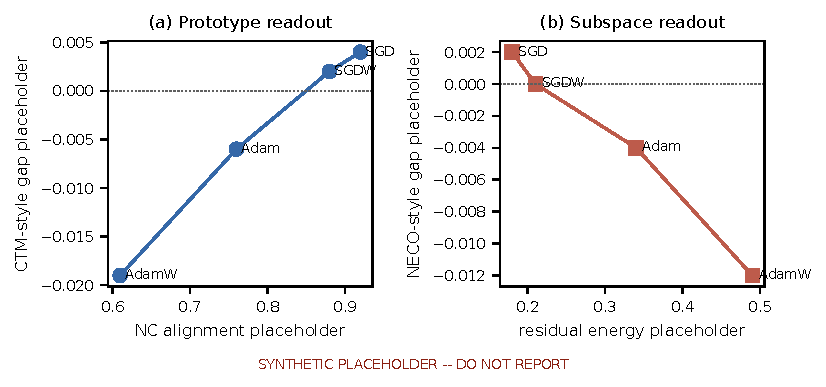
\includegraphics[width=\linewidth]{figures/fig6_prototype_subspace_alignment.pdf}
\caption{SYNTHETIC PLACEHOLDER -- DO NOT REPORT. Placeholder prototype/subspace
diagnostic plot. Values are synthetic placeholders. The intended analysis relates
NC alignment, effective rank, and residual energy to CTM-style, NECO-style,
prototype, and residual-subspace readouts.}
\label{fig:prototype-subspace-alignment}
\end{figure}

Together, the radial, covariance, and subspace controls test whether detector
failures are explained by specific geometry channels or whether they reflect a
broader representation mismatch.

\subsection{Geometry Fingerprints as Detector Diagnostics}
\label{subsec:geometry-fingerprints-detector-diagnostics}

Finally, we ask whether ID-only geometry can guide detector diagnostics before
using OOD validation data. This is a diagnostic goal rather than a claim that ID
geometry fully determines OOD performance. The simplest version is a rule-based
selector: high norm dispersion recommends L2-based controls, poor covariance
conditioning recommends shrinkage or diagonal covariance, strong NC alignment
recommends angular or prototype diagnostics, and large residual energy
recommends PCA or residual-subspace probes.

\begin{table}[t]
\caption{SYNTHETIC PLACEHOLDER -- DO NOT REPORT. Geometry-aware diagnostic
selector. The rules and values are illustrative placeholders only.}
\label{tab:dummy-geometry-selector}
\begin{center}
\footnotesize
\setlength{\tabcolsep}{4pt}
\renewcommand{\arraystretch}{1.15}
\begin{tabular}{@{}p{0.25\textwidth}p{0.26\textwidth}p{0.30\textwidth}p{0.10\textwidth}@{}}
\toprule
ID geometry signal & Suggested diagnostic & Expected compatible family & Dummy hit rate \\
\midrule
High norm dispersion & L2 normalization & L2-Mahalanobis, L2-kNN & 0.78 \\
High covariance condition & Shrinkage / diagonal covariance & GMM, Mahalanobis & 0.71 \\
Strong NC alignment & Angular / prototype readout & CTM-style, prototype cosine & 0.69 \\
High residual energy & PCA / residual probe & NECO-style, PCA residual & 0.64 \\
Mixed geometry profile & Evaluate multiple controls & No single-family recommendation & 0.52 \\
\bottomrule
\end{tabular}
\end{center}
\end{table}


A learned selector can be evaluated after enough architecture--optimizer--seed
cells are available. The target should not be the single best detector on one OOD
dataset. A more stable target is a detector family or control type that remains
competitive across OOD regimes. If the selector fails, then either the fingerprint
\(G(h,W)\) is missing important geometry channels, or OOD severity information is
necessary to choose a detector reliably.

The experiments therefore test both links in the optimizer--geometry--detector
pathway. The interpolation and paired optimizer comparisons test whether
optimizer choice moves the predicted ID geometry channels. The detector-family
and diagnostic-control analyses test whether downstream scores respond according
to their readout channel. The geometry-aware diagnostic analysis tests whether
the same ID fingerprint can be useful before OOD validation.
